\documentclass[9pt, mathserif]{beamer}
\usefonttheme{serif}
\usetheme{Berlin}
\usecolortheme{seagull}
\usepackage[utf8]{inputenc}
\usepackage{amsfonts}
\usepackage{lmodern}
\usepackage{amsmath}
\usepackage{geometry}
\usepackage{graphicx}
\usepackage{tikz}
\usepackage{tikz-feynman}
\usepackage{url}
\usepackage{geometry}
\usepackage{bm}
\usepackage{physics}
\usepackage{float}
\usepackage{wrapfig}
\usepackage{multirow}
\usepackage{xcolor}
\usepackage{indentfirst}
\usepackage{multicol}
\usepackage{ragged2e}
\usepackage{subcaption}
\setlength{\parindent}{2em}


\title{\textbf{\textbf{A Fundemental Study on Photon Isolation}}}
\author{\textbf{Song Xianglong}}
\institute{Boling Class of Physics, School of Physics, Nankai University, Tianjin 300071, China}
\date{\today}

\begin{document}
\justifying
    \begin{frame}
        \titlepage
    \end{frame}
    \begin{frame}
		\frametitle{Contents} 
        \tableofcontents
	\end{frame}
    \section{Introduction}
        \begin{frame}
            In Quantum Electrodynamics (QED), splitting refers to a process where a high-energy particle emits or dacays a daughter 
	        particle and undergoes a change in its state.\par
            \begin{wrapfigure}{l}{0.6\textwidth}
                \centering
                \begin{tikzpicture}
                    \begin{feynman}
                        \vertex (a) {\(q\)};
                        \vertex [right=of a] (b) ;
                        \vertex [above right=of b] (f1) {\(\gamma\)};
                        \vertex [below right=of b] (c) {\(q\)};
                        \diagram* {
                          (a) -- [fermion] (b) -- [photon] (f1),
                          (b) -- [fermion] (c),
                        };
                      \end{feynman}
                \end{tikzpicture}
                \caption{Feynman diagram for \(q \rightarrow q\gamma\).}
                \label {fig:feynman}
            \end{wrapfigure}
            Here we are interested in  $q\rightarrow q\gamma$ process.\par
            The probability for a quark to radiate a photon with some angle $\theta_{\gamma}$ and momentum fraction $z_{\gamma}$ is given by:
	        \begin{equation}    
                \begin{aligned}
                    \dd P_{q\rightarrow q\gamma}=\frac{\alpha_ee^2}{2\pi}\frac{\dd \theta_{\gamma}}{\theta_{\gamma}}P(z_{\gamma})\dd z_{\gamma},\\
                    P(z)=\left(\frac{1+(1-z)^2}{z}\right)_+,
                \end{aligned}
            \end{equation}
        \end{frame}
    
    
    \section{Grooming}
        \begin{frame}
            Jet grooming refers to a set of techniques used to improve the reconstruction and analysis of jets. Jets can be affected by various effects, such as soft radia- tion and pileup, which can lead to a broader or less well-defined jet structure. Grooming methods help mitigate these effects and enhance the precision of jet measurements.
        \end{frame}
        \subsection{Soft Drop Algorithm}
            \begin{frame}
                Soft Drop is a grooming algorithm that involves recursively declustering a jet into two subjets and rejecting the subjet with the lower momentum if certain conditions are not met.\par
                Soft drop declustering is used to identify hard subjets within a jet that satisfy the condition:
		        \begin{equation}
			        \frac{\min(p_{T1},p_{T2})}{p_{T1}+p_{T2}}\geq z_{\mathrm{cut}}\left(\frac{R_{12}}{R_0}\right)^{\beta},
		        \end{equation}
            \end{frame}
    
            
    \section{Photon Isolation}
        \subsection{Procedure}
            \begin{frame}
                The photon isolation procedure is a combination of soft drop declustering and soft drop isolation.
                \begin{itemize}
                    \item $R=0.4$, ankt-$k_T$ algorithm
                    \item soft drop declustering: $z_{\mathrm{cut}}=0.1$, $\beta=0$, $R_0=R=0.4$
                    \item soft drop isolation: $z_{\mathrm{cut}}=0.1$, $\beta=2$, $R_0=R_{12}/2$
                \end{itemize}
            \end{frame}
        \subsection{Some Observables}
            \begin{frame}
                \frametitle{$z_{\mathrm{iso}}$}
                Isolated photon momentum sharing:
                \begin{equation}
                    z_{\mathrm{iso}}=\frac{p_{T\gamma-\mathrm{sub}}}{p_{T\gamma-\mathrm{sub}}+p_{T\mathrm{had}-\mathrm{sub}}}.
                \end{equation}
            \end{frame}
            \begin{frame}
                \frametitle{$\theta$}
                $\theta$ denotes the angular distance between two objects in the $\eta-\phi$ plane,
                \begin{equation}
                    \Delta R_{12}=\sqrt{(\Delta \eta)^2+(\Delta \phi)^2}.
                \end{equation}
            \end{frame}


    \section{Parton Shower Study}
        \begin{frame}
            For event selection, we require $p_{T\mathrm{jet}}>350\mathrm{~GeV}$ as a defult setting.
            \begin{figure}[t]
                \centering
                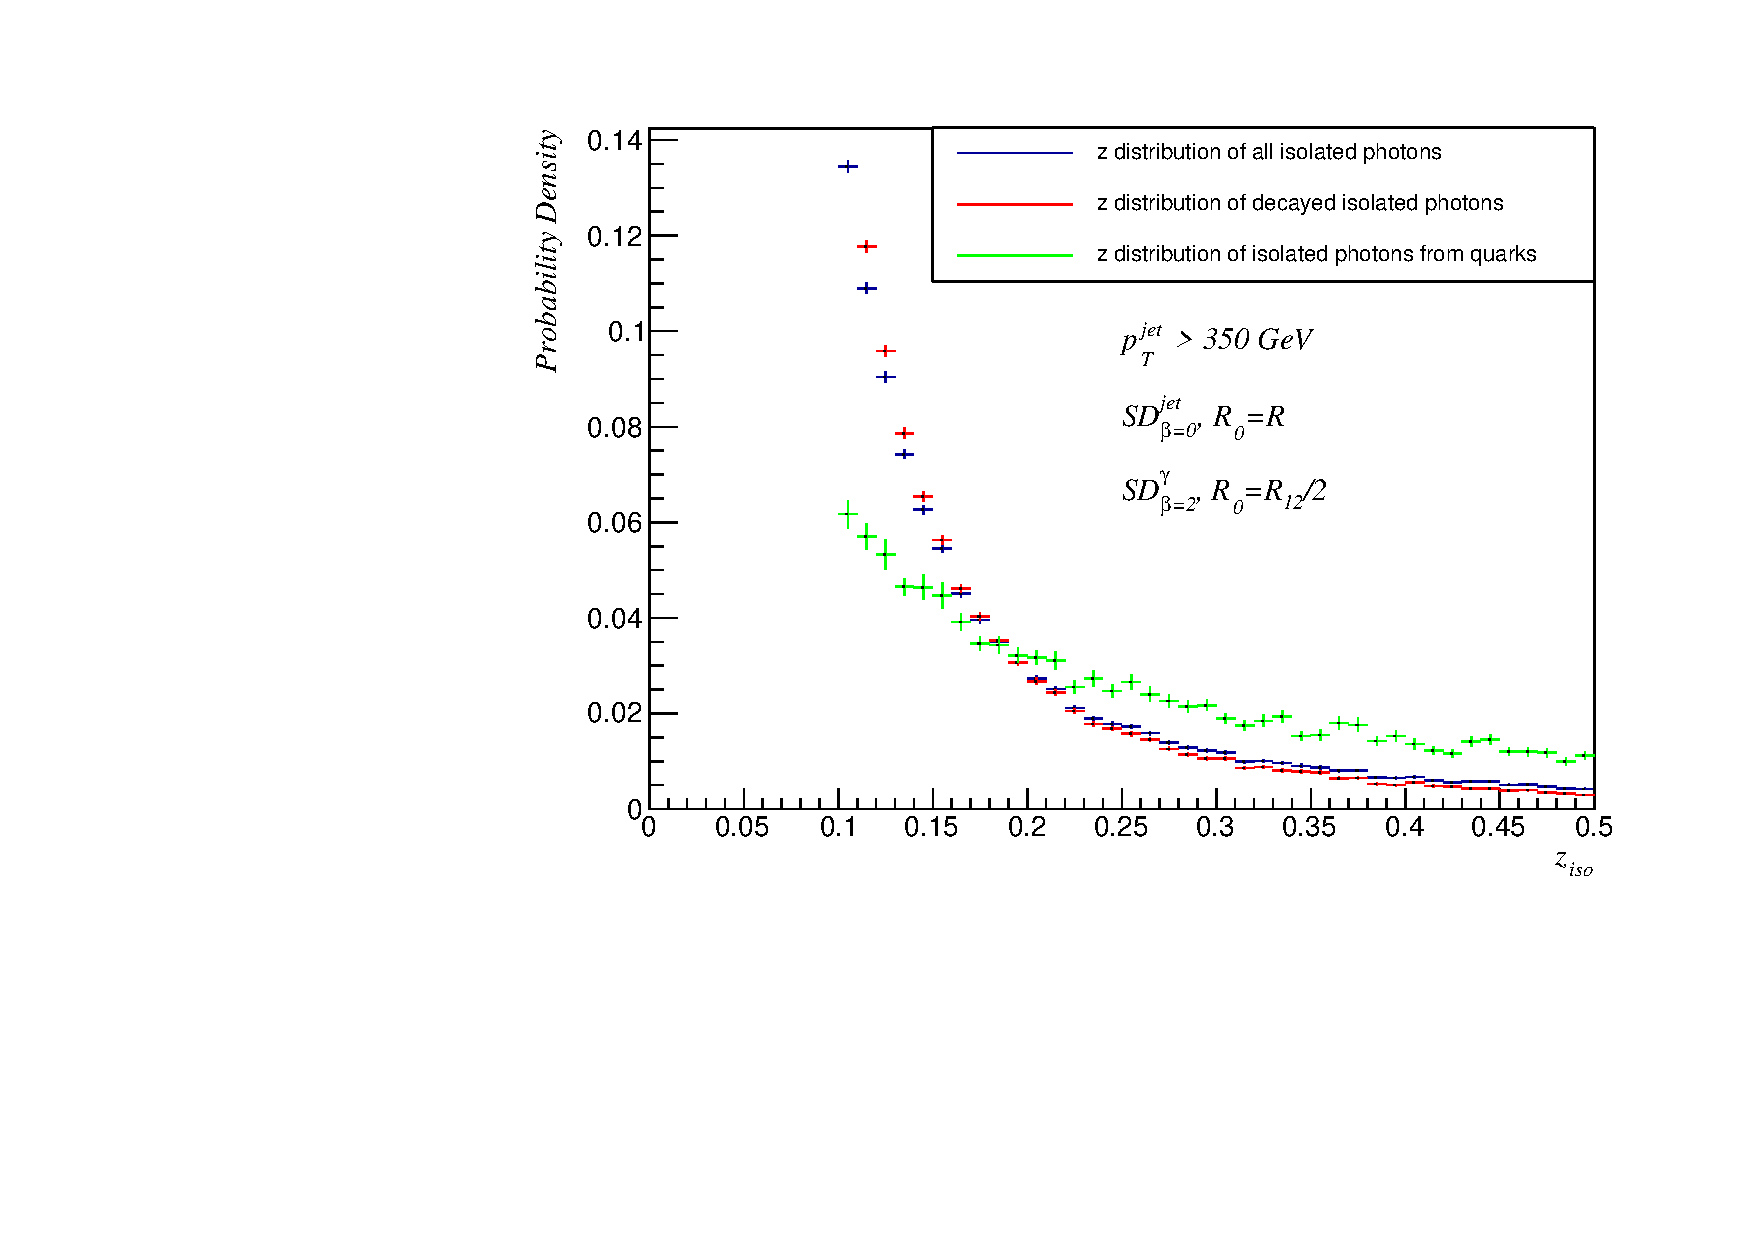
\includegraphics[width=0.6\linewidth]{1.pdf}
                \caption{All isolated photons without $\theta_{\mathrm{cut}}$}
            \end{figure}
            Here we show the $z$ distribution of all isolated photons ($p_{T\mathrm{jet}}>350\mathrm{~GeV}$).
        \end{frame}
        \begin{frame}
            \begin{figure}[t]
                \centering
                \begin{subfigure}{0.47\linewidth}
                    \centering
                    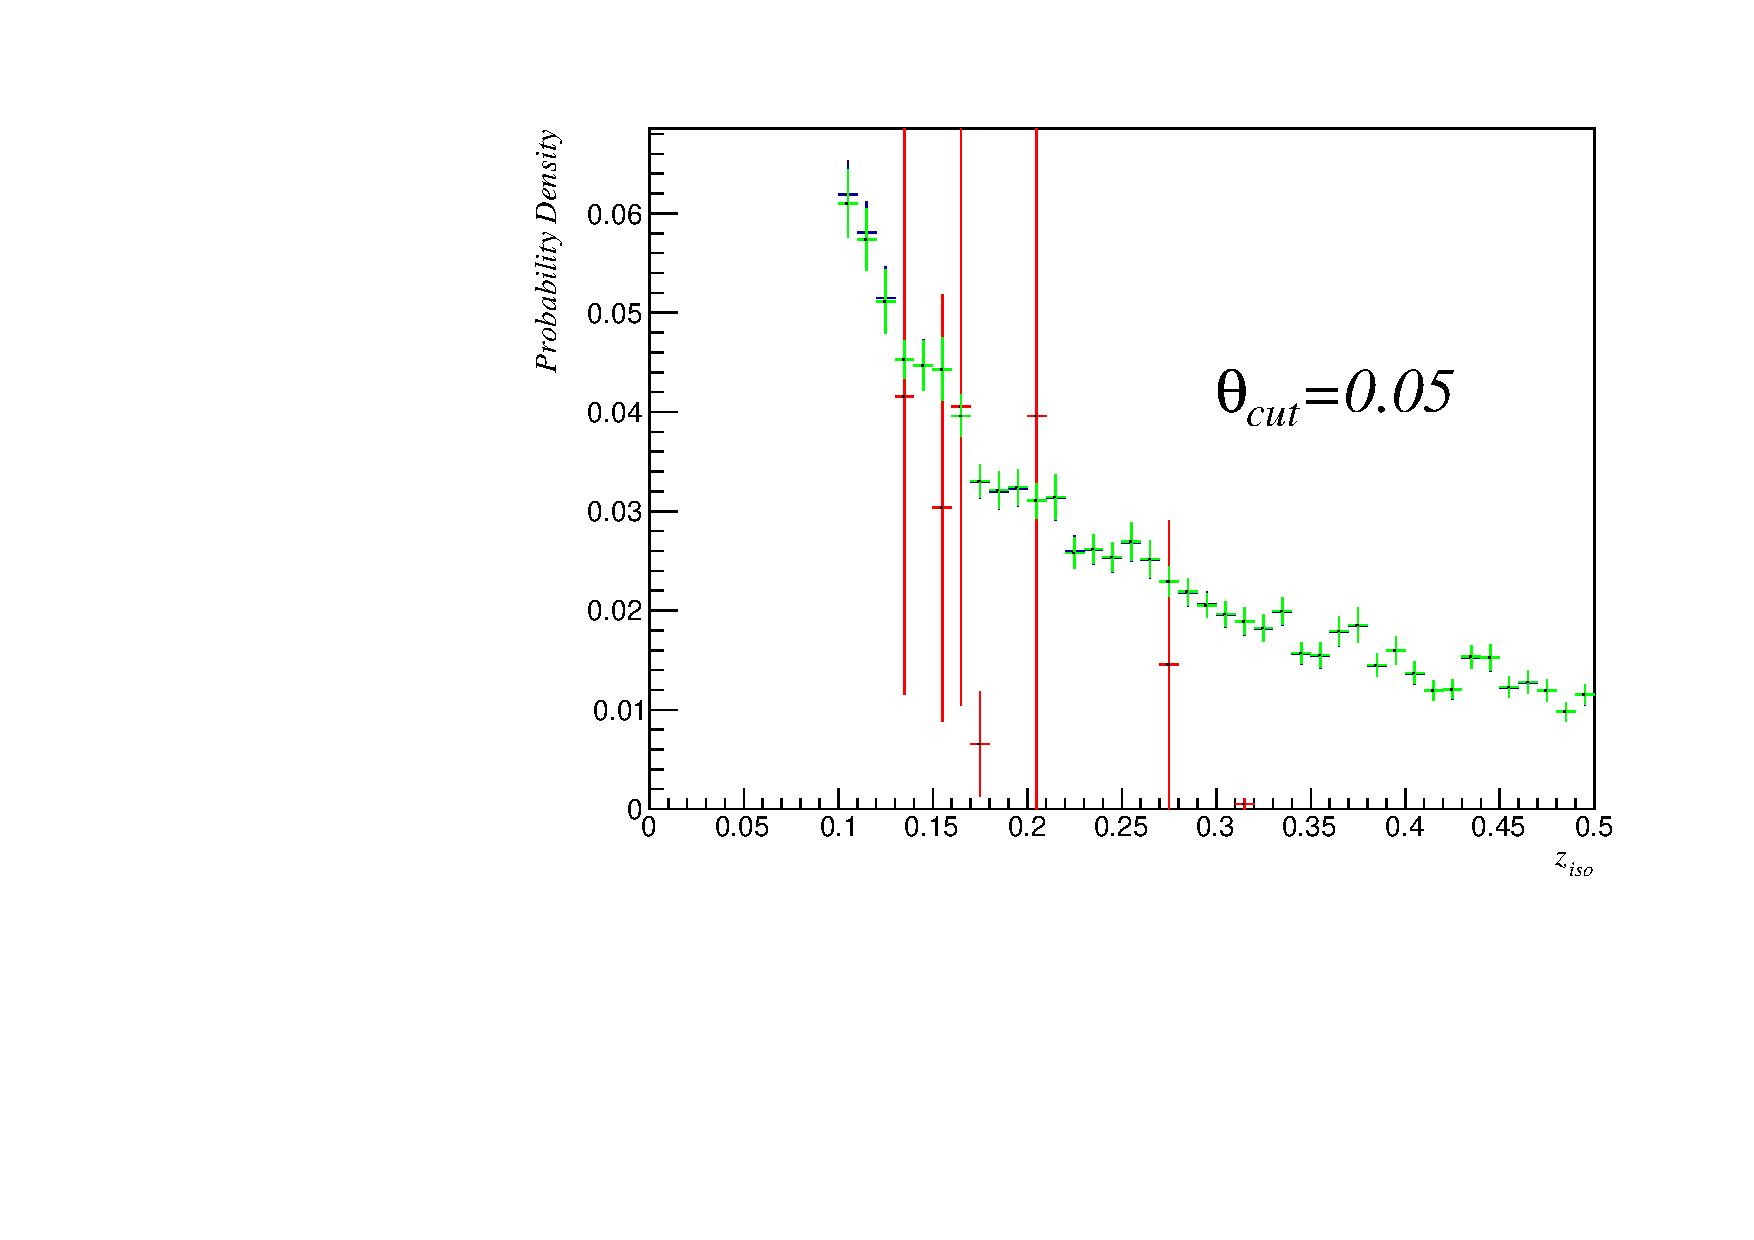
\includegraphics[width=\linewidth]{2.pdf}
                    \caption{}
                \end{subfigure}
                \begin{subfigure}{0.47\textwidth}
                    \centering
                    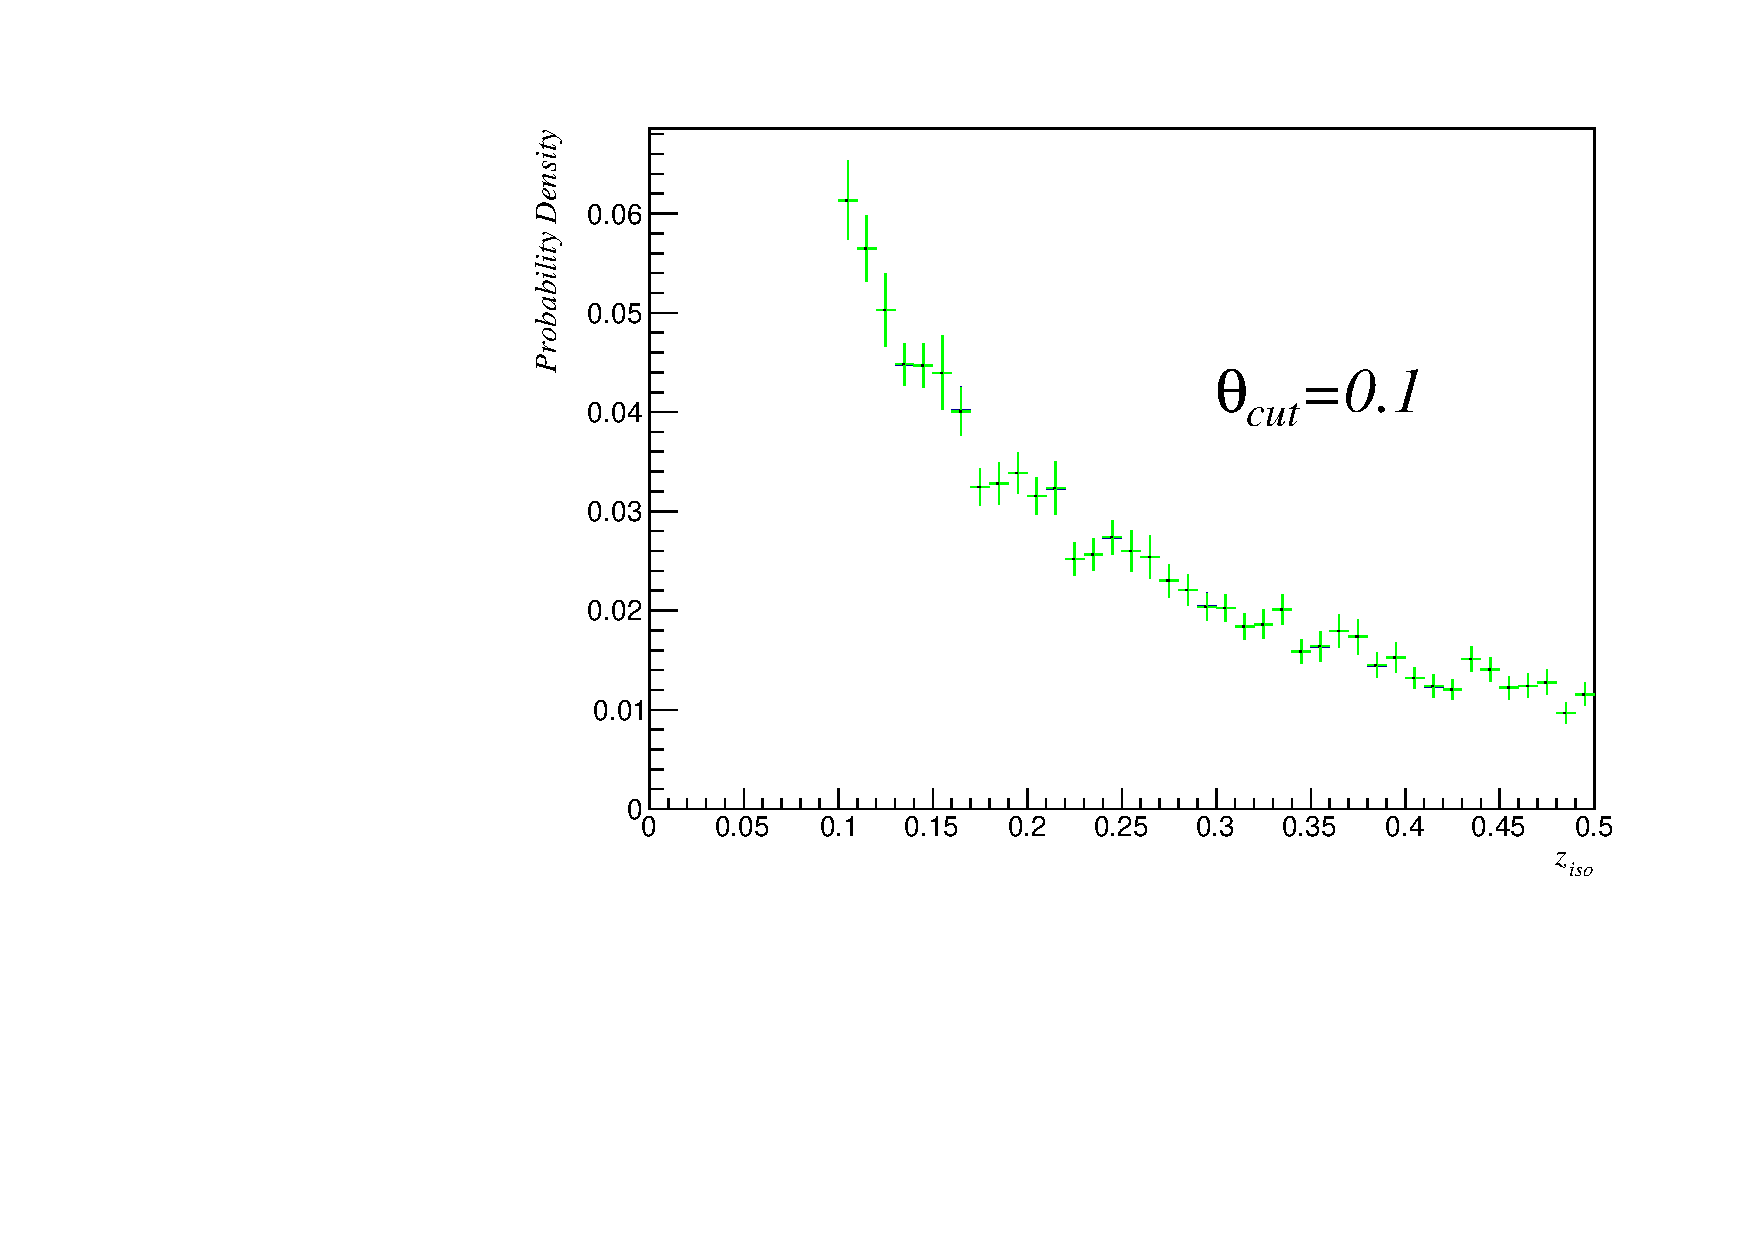
\includegraphics[width=\linewidth]{3.pdf}
                    \caption{}
                \end{subfigure}
                \caption{$z$ distribution with $\theta_{\mathrm{cut}}$}
            \end{figure}
            Here we set a $\theta_{\mathrm{cut}}$ to be 0.05. And when increase the $\theta_{\mathrm{cut}}$ to 0.1,
		    there are no splittings from meson decay.
        \end{frame}
        \begin{frame}
            \begin{figure}
                \centering
                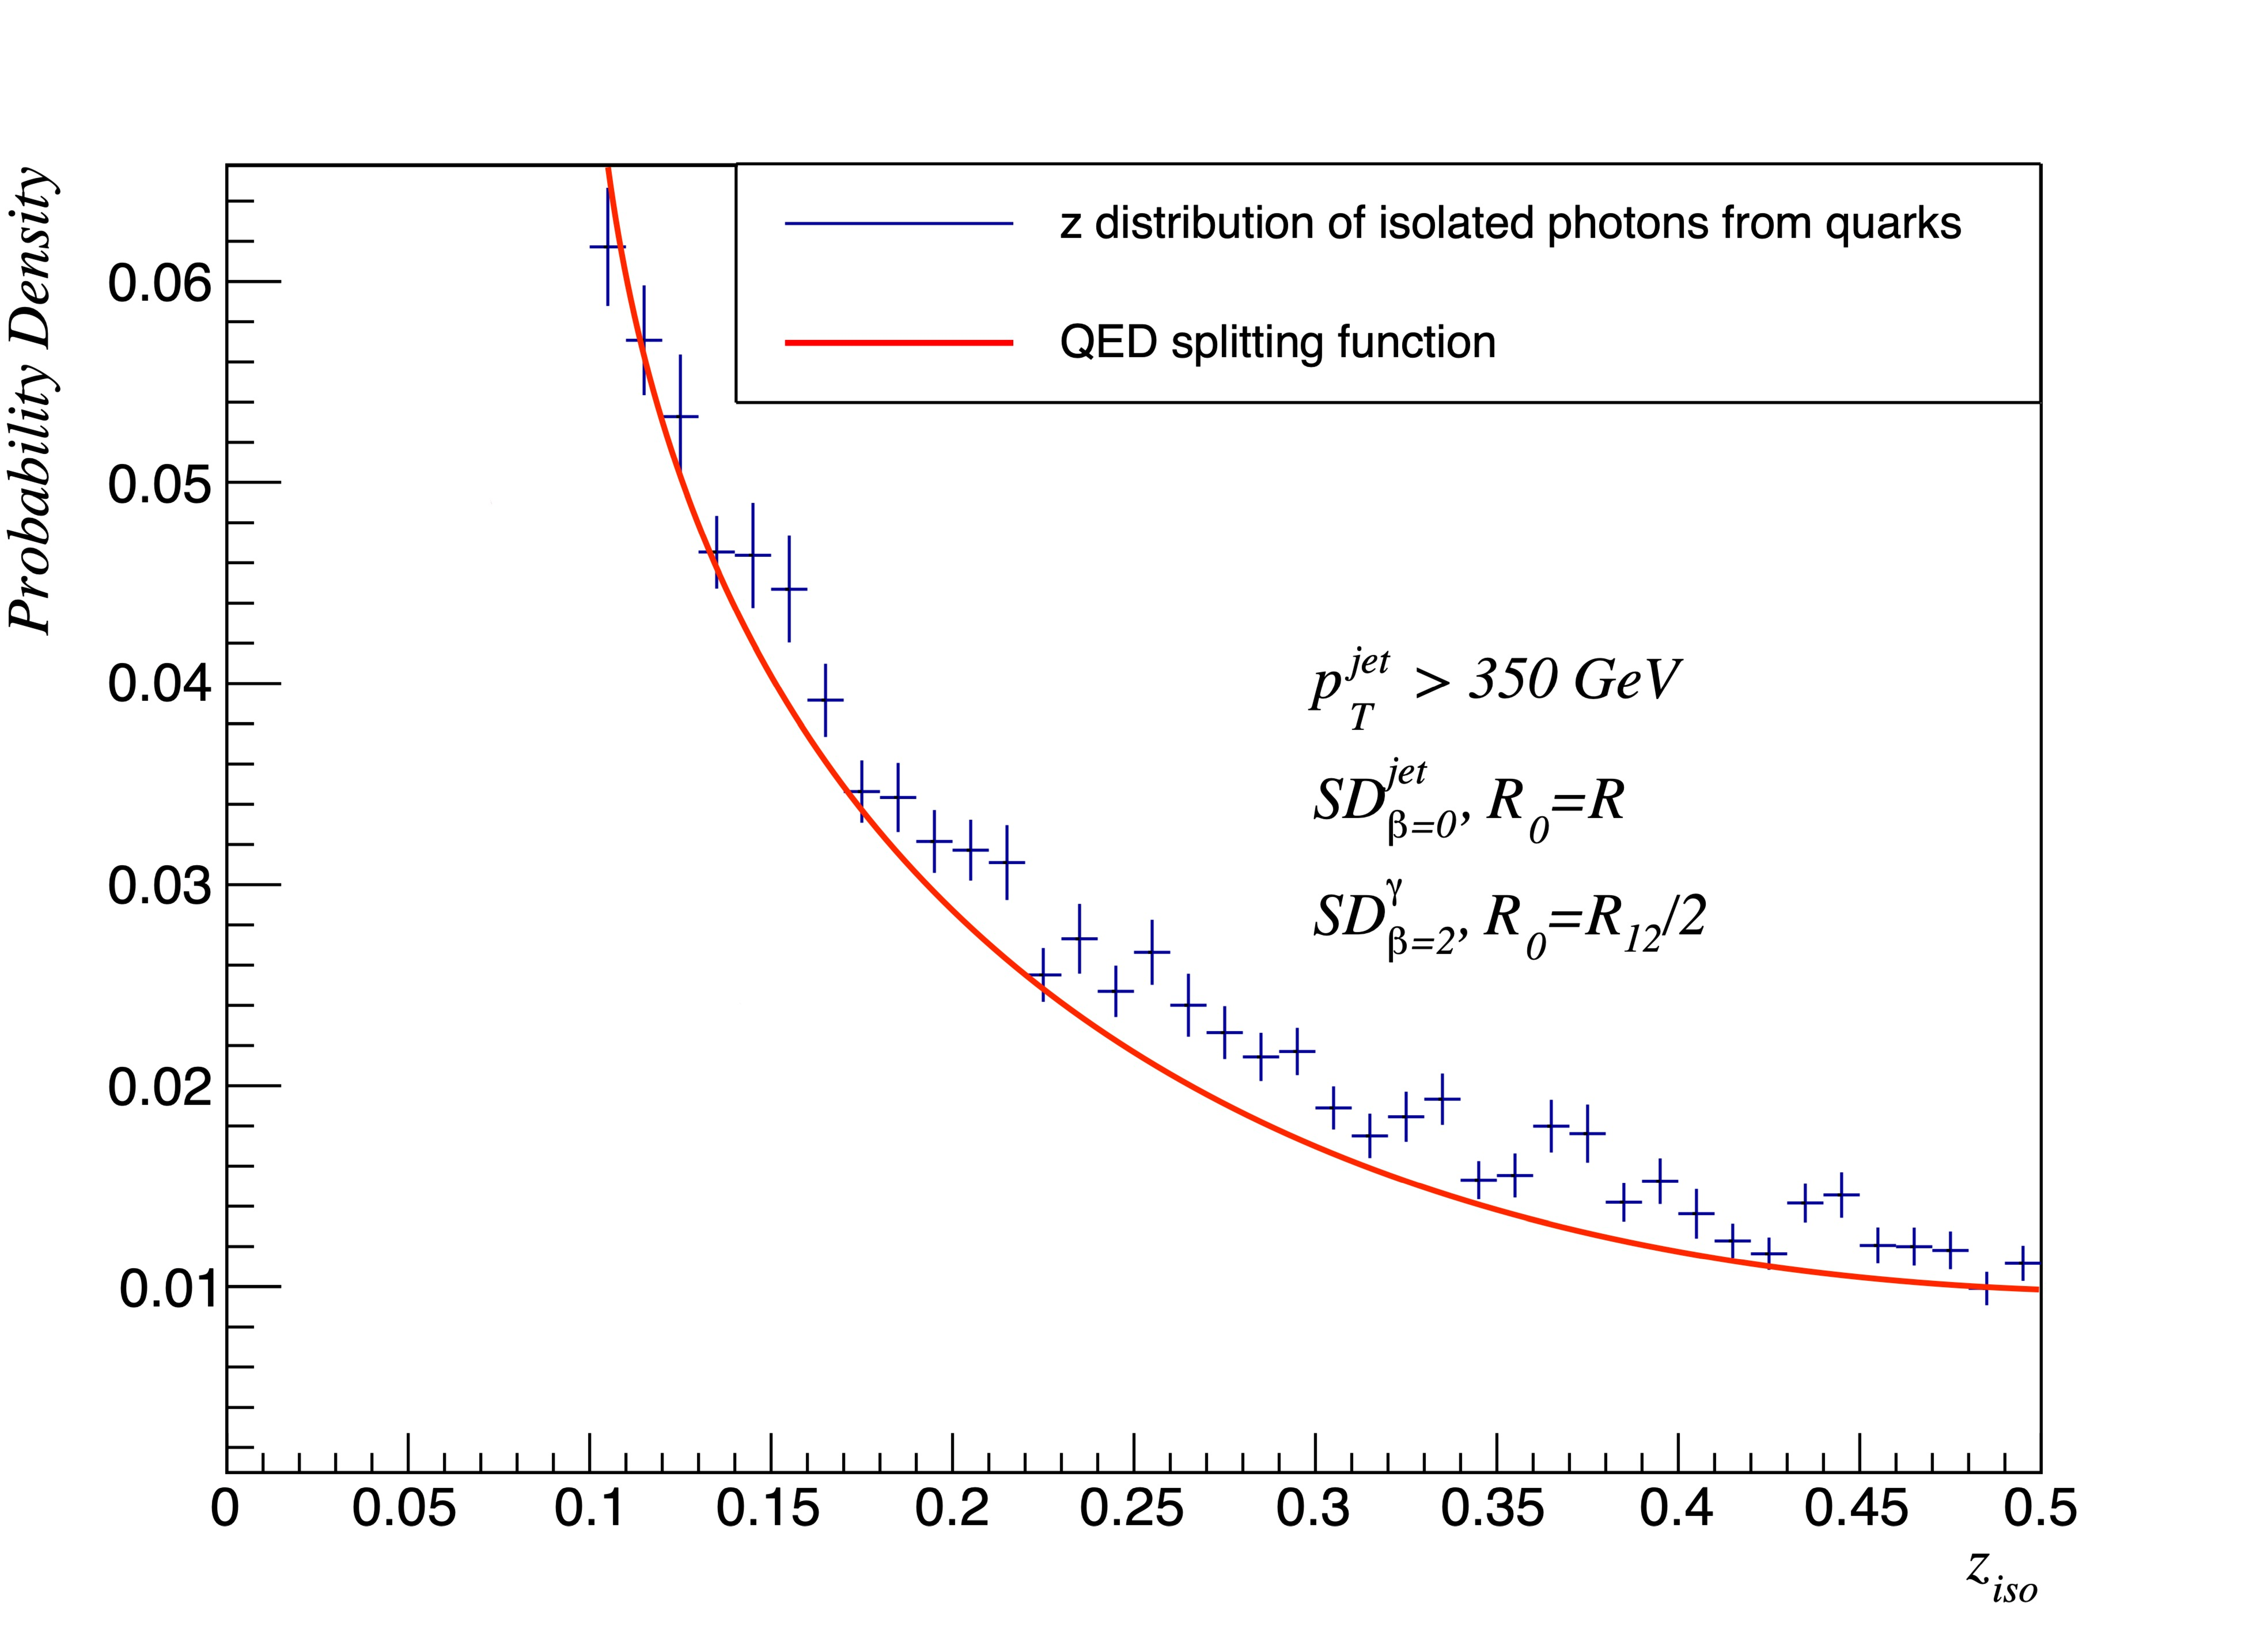
\includegraphics[width=0.6\linewidth]{5.pdf}
                \caption{QED splitting function and isolated photons from quarks}
            \end{figure}
            Here we plot the QED splitting function with $z$ distribution of quark photons.
        \end{frame}



\end{document}